\documentclass{standalone}
\usepackage[dvipsnames]{xcolor}

\usepackage{tikz}
\usetikzlibrary{shapes.geometric}

\tikzset{
    cross/.pic = {
    \draw[rotate = 45] (-#1,0) -- (#1,0);
    \draw[rotate = 45] (0,-#1) -- (0, #1);
    }
}
\tikzset{
    InvertedTri/.style={
        draw,
        shape border rotate=-90,
        isosceles triangle,
        isosceles triangle apex angle=60,
        fill=green,
        node distance=2cm,
        minimum height=2em
    }
}

\tikzset{
    NormalTri/.style={
        draw,
        shape border rotate=90,
        isosceles triangle,
        isosceles triangle apex angle=60,
        fill=red,
        node distance=2cm,
        minimum height=2em
    }
}
\tikzset{
    square/.style={regular polygon,regular polygon sides=4, fill=cyan,
    minimum height=3em}
}

\newcommand{\drawMax}[1]{\node[NormalTri]  at #1 {}}
\newcommand{\drawMin}[1]{\node[InvertedTri]  at #1 {}}
\newcommand{\drawNode}[2]{\node[square] at #1 {#2}}
\begin{document}
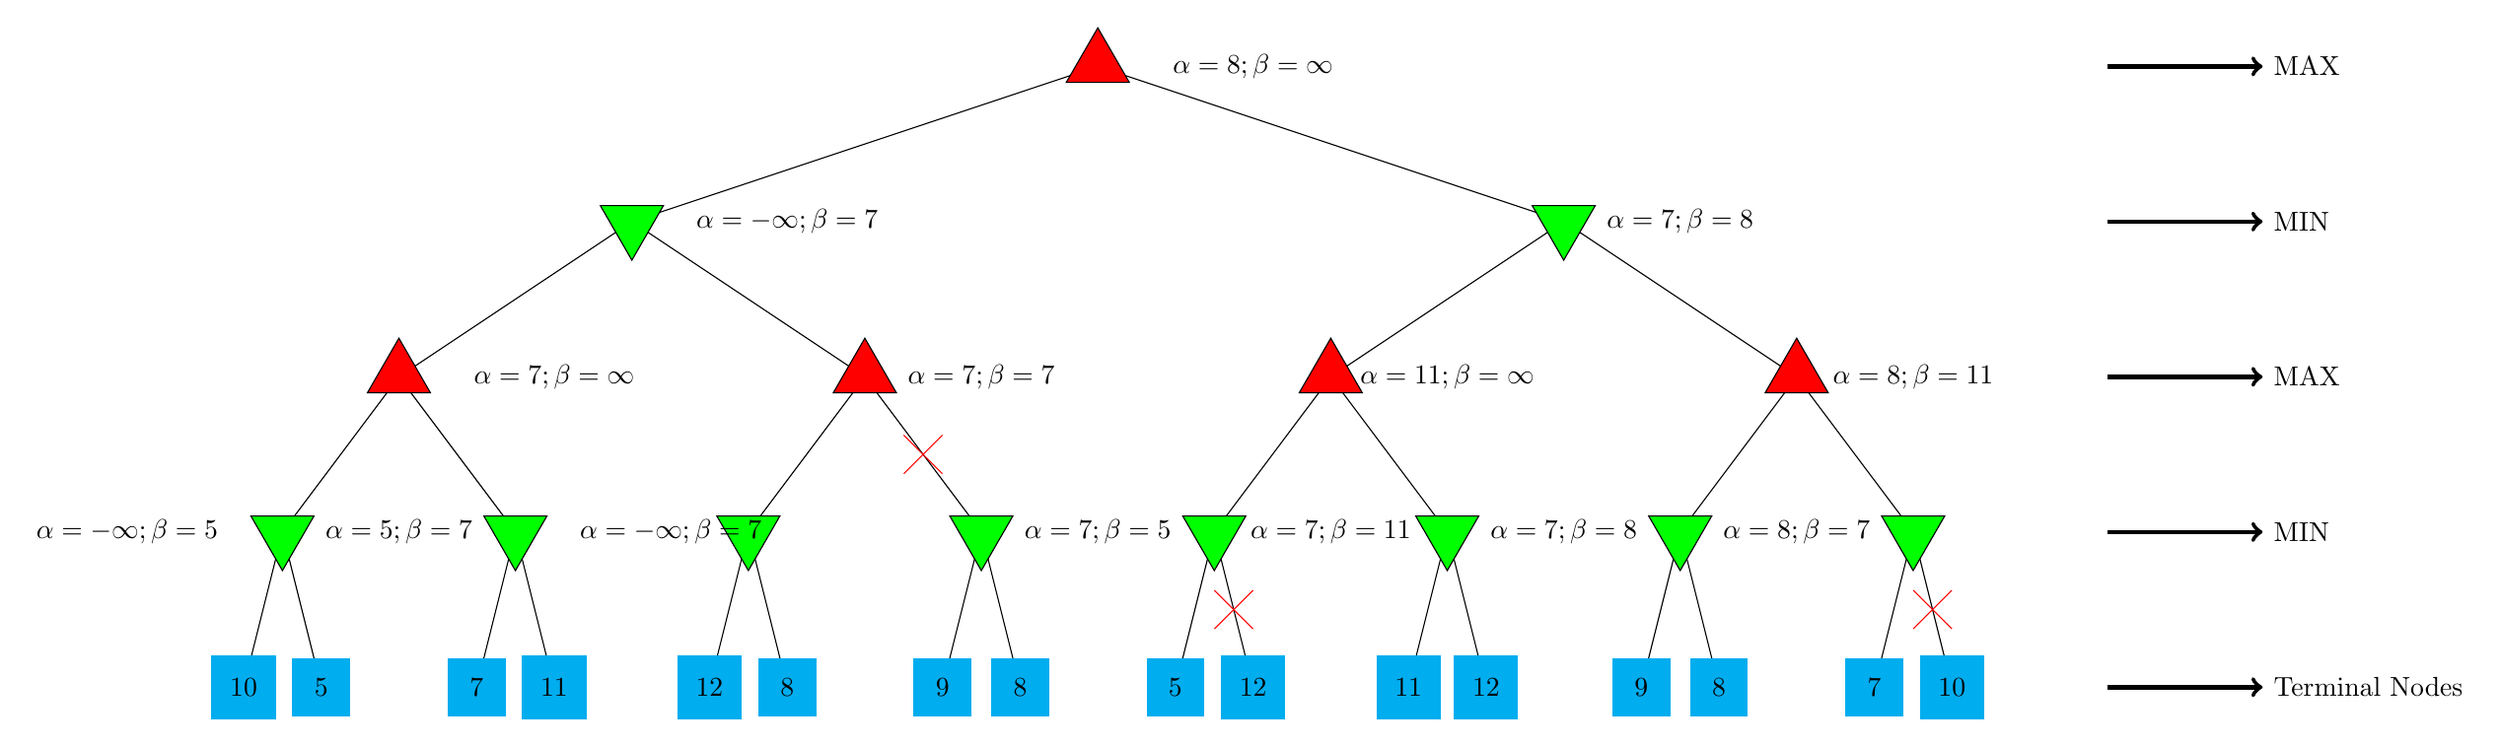
\begin{tikzpicture}



    \draw (0,0) -- (-6,-2);

    \draw (-6,-2) -- (-9,-4);
    \draw (-6,-2) -- (-3,-4); 

    \draw (-9,-4) -- (-10.5,-6); 
    \draw (-9,-4) -- (-7.5,-6);

    \draw (-3,-4) -- (-4.5,-6);
    \draw (-3,-4) -- (-1.5,-6); 

    \draw (-10.5,-6) -- (-11,-8); 
    \draw (-10.5,-6) -- (-10,-8);

    \draw (-7.5,-6) -- (-8,-8); 
    \draw (-7.5,-6) -- (-7,-8); 

    \draw (-4.5,-6) -- (-5,-8); 
    \draw (-4.5,-6) -- (-4,-8);

    \draw (-1.5,-6) -- (-2,-8); 
    \draw (-1.5,-6) -- (-1,-8);

    \draw (0,0) -- (6,-2);  
    
    \draw (6,-2) -- (3,-4);
    \draw (6,-2) -- (9,-4);

    \draw (3,-4) -- (1.5,-6);
    \draw (3,-4) -- (4.5,-6);
    \draw (9,-4) -- (7.5,-6); 
    \draw (9,-4) -- (10.5,-6);

    \draw (1.5,-6) -- (1,-8);
    \draw (1.5,-6) -- (2,-8);

    \draw (4.5,-6) -- (4,-8);
    \draw (4.5,-6) -- (5,-8); 

    \draw (7.5,-6) -- (7,-8); 
    \draw (7.5,-6) -- (8,-8); 


    \draw (10.5,-6) -- (10,-8);
    \draw (10.5,-6) -- (11,-8);


    \drawMax{(0,0)};
    \node at (2,0) {$\alpha=8 ; \beta=\infty$};

    \drawMin{(-6,-2)};
    \node at (-4,-2) {$\alpha=-\infty ; \beta=7$};

    \drawMax{(-9,-4)};
    \node at (-7,-4) {$\alpha=7; \beta=\infty$};
    \drawMax{(-3,-4)};
    \node at (-1.5,-4) {$\alpha=7; \beta=7$};


    \drawMin{(-10.5,-6)};
    \node at (-12.5,-6) {$\alpha=-\infty ; \beta=5$};
    \drawMin{(-7.5,-6)};
    \node at (-9,-6) {$\alpha=5; \beta=7$};

    \drawMin{(-4.5,-6)};
    \node at (-5.5,-6) {$\alpha=-\infty ; \beta=7$};
    \drawMin{(-1.5,-6)};

    \drawNode{(-11,-8)}{10};
    \drawNode{(-10,-8)}{5};

    \drawNode{(-8,-8)}{7};
    \drawNode{(-7,-8)}{11};

    \drawNode{(-5,-8)}{12};
    \drawNode{(-4,-8)}{8};

    \drawNode{(-2,-8)}{9};
    \drawNode{(-1,-8)}{8};


    \drawMin{(6,-2)};  
    \node at (7.5,-2) {$\alpha=7 ; \beta=8$};

    \drawMax{(3,-4)};
    \node at (4.5,-4) {$\alpha=11 ; \beta=\infty$};
    \drawMax{(9,-4)};  
    \node at (10.5,-4) {$\alpha=8 ; \beta=11$};

    \drawMin{(1.5,-6)};
    \node at (0,-6) {$\alpha=7 ; \beta=5$};
    \drawMin{(4.5,-6)};
    \node at (3,-6) {$\alpha=7 ; \beta=11$};

    \drawMin{(7.5,-6)};
    \node at (6,-6) {$\alpha=7 ; \beta=8$};
    \drawMin{(10.5,-6)};
    \node at (9,-6) {$\alpha=8 ; \beta=7$};

    \drawNode{(1,-8)}{5};
    \drawNode{(2,-8)}{12};

    \drawNode{(4,-8)}{11};
    \drawNode{(5,-8)}{12};    

    \drawNode{(7,-8)}{9};
    \drawNode{(8,-8)}{8};

    \drawNode{(10,-8)}{7};
    \drawNode{(11,-8)}{10};


    \draw[->,ultra thick] (13,0) -- (15,0) node [right]{MAX};
    \draw[->,ultra thick] (13,-2) -- (15,-2) node [right]{MIN};
    \draw[->,ultra thick] (13,-4) -- (15,-4) node [right]{MAX};
    \draw[->,ultra thick] (13,-6) -- (15,-6) node [right]{MIN};
    \draw[->,ultra thick] (13,-8) -- (15,-8) node [right]{Terminal Nodes};

    \path (-2.25,-5) pic[red] {cross=10pt};
    \path (1.75,-7) pic[red] {cross=10pt};
    \path (10.75,-7) pic[red] {cross=10pt};

\end{tikzpicture}
\end{document}


